\chapter{研究背景}\label{chap:background}

本章では、本研究の背景について述べる。

\section{コンピュータプログラムと人}\label{ux30b3ux30f3ux30d4ux30e5ux30fcux30bfux30d7ux30edux30b0ux30e9ux30e0ux3068ux4eba}

コンピュータプログラムとは、コンピュータに実行させたい一連の処理手順を記述したものである。
コンピュータはこのプログラムに記述された処理を解釈し、実行する。

コンピュータプログラムの実行対象はコンピュータであるが、人が実行するプログラムも存在する。
マニュアルやレシピといった、人間にとっての手順書だ。
人間は手順書に書いてある内容に沿って行動し、目的を達成する。
例えば、何か料理を作りたいときなどは、料理のレシピを見ながら、そこに記述されている内容を自分で解釈し、実行する。

コンピュータにとってのプログラムと人にとってのプログラムには類似性がある。
双方ともに、実行する処理について記述されたものである。
例えば、料理のレシピをコンピュータプログラムのような記述するならば、図\ref{fig:background_cooking}のようになる。

\begin{figure}[htbp]
  \begin{center}
  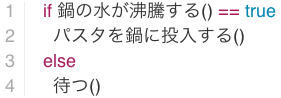
\includegraphics[width=.4\linewidth,bb=0 0 281 98]{images/background_cooking.js.png}
  \end{center}
  \caption{料理レシピをコンピュータプログラム風に記述する}
  \label{fig:background_cooking}
\end{figure}

また、小売店の店員マニュアルであれば、図\ref{fig:background_retail}のようになる

\begin{figure}[htbp]
  \begin{center}
  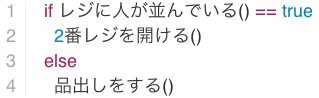
\includegraphics[width=.4\linewidth,bb=0 0 319 98]{images/background_retail.js.png}
  \end{center}
  \caption{料理レシピをコンピュータプログラム風に記述する}
  \label{fig:background_retail}
\end{figure}

このように、人間にとっての処理もコンピュータにとっての処理も、同じような記法で記述することが可能である。
しかし、両者の処理を統合して記述するための仕組みは存在しない。

\section{プログラムの処理領域の拡張}\label{ux30d7ux30edux30b0ux30e9ux30e0ux306eux51e6ux7406ux9818ux57dfux306eux62e1ux5f35}

プログラムによって制御を記述できるような領域はどんどん広がっている。
近年では、Arduino\footnote{http://www.arduino.cc/}やRaspberryPi\footnote{http://www.raspberrypi.org/}等の登場によって、
誰でも非常に簡単にセンサーやアクチュエータを扱えるようになっている。
その制御を記述するのはプログラムである。
また、建築物の構成要素をプログラマブルにする試み\cite{squama}や、プログラムによってその構成を動的に変化させるモジュールについての研究もなされている。
より高性能なロボットの登場によって、今まで人間がやっていたような領域においても、プログラムの制御が有効に働くようになるだろう。
今後、プログラムによる制御は更に広がり、あらゆる制御をプログラムで記述するようになっていくのではないかと考えられる。

\section{プログラムの実行対象}\label{ux30d7ux30edux30b0ux30e9ux30e0ux306eux5b9fux884cux5bfeux8c61}

コンピュータプログラムに書かれた処理でも、コンピュータ以外がその処理を実行するといった事例も多く存在している。
コンピュータは優れた処理能力を持つが、認識能力などの分野においてはまだ人間のほうが優れた能力を持っている。
これらのような、コンピュータのみでは実現が困難な処理を、人間を計算資源として組み込み利用することによって
解決しようという概念はヒューマンコンピュテーション\cite{humancomputation}と呼ばれる。

インターネットを介した不特定多数の人間に仕事を依頼する仕組みはクラウドソーシングと呼ばれる。
クラウドソーシングにおいてもヒューマンコンピュテーションが適応され、大量の人を計算資源とした処理が安価で実現されている。

ヒューマンコンピュテーションやクラウドソーシングの事例から、人間はリソースとして捉えることが出来る。
人間であろうとコンピュータであろうと、処理結果を得ることが出来れば良い。
プログラムにとって、人間もコンピュータも処理を実行するためのリソースであると言える。

\section{あらゆる処理をプログラムで記述する}\label{ux3042ux3089ux3086ux308bux51e6ux7406ux3092ux30d7ux30edux30b0ux30e9ux30e0ux3067ux8a18ux8ff0ux3059ux308b}

プログラムが記述できる世界は広がっている。
コンピュータの中だけでなく、実世界の制御など、あらゆる処理を記述するようになっている。
プログラムは、対象を限定しない汎用的な処理記述フォーマットであると言える。

また、プログラムで記述された処理の実行リソースもコンピュータだけに限定されない。
前項の通り、人間さえも実行リソースとして利用されるようになっている。
今後、プログラムにおける人間とコンピュータの境界はあいまいになっていくと考えられる。
コンピュータと人間が処理を実行するリソースとして対等であるならば、
プログラム上においてもコンピュータと人間への指示は同じように記述されるべきである。

このように、プログラムの処理領域と処理実行対象は拡張されている。
拡張されたことによって、
人間とコンピュータの両方を処理実行対象として、あらゆる処理や手順、行動をプログラムとして記述するようなことが可能となる。
そもそも人間とコンピュータでは、得意な分野や出来ることが異なる。
人間は柔軟な思考能力や身体を所有することから、パターン認識や感性判断の必要な処理、実世界への干渉が得意である。
また、意思決定は基本的に人間が担うべき処理である。
コンピュータは高速な演算能力を所有することから、計算や記憶、正確なセンシングなどを担うべきである。
人間とコンピュータは、ある実現したい処理があれば、それを実現するために、お互いが機能を補い合うべきだ。
こうして、人間とコンピュータが協力しあうことによって、今までには実現しなかったような処理を実現可能となる。
例えば、人間のタスクである「料理をする」という行動さえも、プログラムで記述できるようになる。

このような世界を実現出来れば非常に面白く、プログラムの可能性が更に広がる。
人間とコンピュータへの指示を同じ記法で実現できれば、非常に面白い。
だが、現状では部分的にしか実現できていない。
プログラムから人間をリソースとして活用する仕組みは、クラウドソーシングやヒューマンコンピュテーションといった、計算資源として利用している。
知的労働以外への応用をプログラムレベルでjつげんすることはできていない。
また、クラウドソーシング等の場合、インターネットを介した不特定の人間を対象としたものである。
自分の家で、自分の日常行動をプログラムにしたいとき等は、自分自身を対象として指定できなくてはならない。
また、家族等の身内にしか実行してほしくない処理の内容も存在する。

コンピュータと人間への指示を融合させたプログラミングが可能な環境を実現することによって、非常に面白いプログラミングが可能になる。

\section{まとめ}\label{ux307eux3068ux3081}

本章では、プログラムの現状について示し、人間とコンピュータが対等な処理実行のリソースであるということを示した。
また、プログラムが実行対象を選ばない汎用的な処理記述フォーマットであることを示し、あらゆる処理を記述するためのプログラミング環境の実現に向けた
状況を考察した。
